\documentclass[border=2pt]{standalone}
\usepackage[utf8]{inputenc} % Required for inserting images
\usepackage{tikz}
\usepackage{helvet}
\usetikzlibrary{shapes.geometric, arrows}
\pagecolor{white}

%-------------------------defining colorblind friendly colors
% Using pale color scheme in Figure 6
% by Paul Tol https://personal.sron.nl/~pault/
\definecolor{cbblue}{HTML}{BBCCEE}
\definecolor{cbcyan}{HTML}{CCEEFF}
\definecolor{cbgreen}{HTML}{CCDDAA}
\definecolor{cbyellow}{HTML}{EEEEBB}
\definecolor{cbred}{HTML}{FFCCCC}
\definecolor{cbgrey}{HTML}{DDDDDD}

% -------------------------defining nodes
\tikzstyle{input} = [trapezium, trapezium left angle =80, trapezium right angle = 100,
minimum width= 3cm, minimum height=0.5cm, text centered, draw=black, fill=cbblue]
\tikzstyle{process} = [rectangle, minimum width = 3cm, minimum height = 1cm,
text centered, , text width=4cm,draw=black, fill=cbgrey]
\tikzstyle{decision} = [diamond, minimum width = 3cm, minimum height = 1cm,
text centered, , text width=3cm, draw=black, fill=cbcyan]
\tikzstyle{changeclass} = [rectangle, rounded corners, minimum width=3cm, minimum height=1cm,
text centered, draw = black, fill=cbyellow]
\tikzstyle{reject} = [trapezium, trapezium left angle =80, trapezium right angle = 100,
minimum width= 1cm, minimum height=0.5cm, text centered, draw=black, fill=cbred]
\tikzstyle{accept} = [trapezium, trapezium left angle =80, trapezium right angle = 100,
minimum width= 1cm, minimum height=0.5cm, text centered, draw=black, fill=cbgreen]

% -------------------------defining connectors
\tikzstyle{arrow} = [thick,->, >=stealth]
\tikzstyle{line} = [thick,-,>=stealth]
\begin{document}

% ------------------------- tikz image (flow chart)
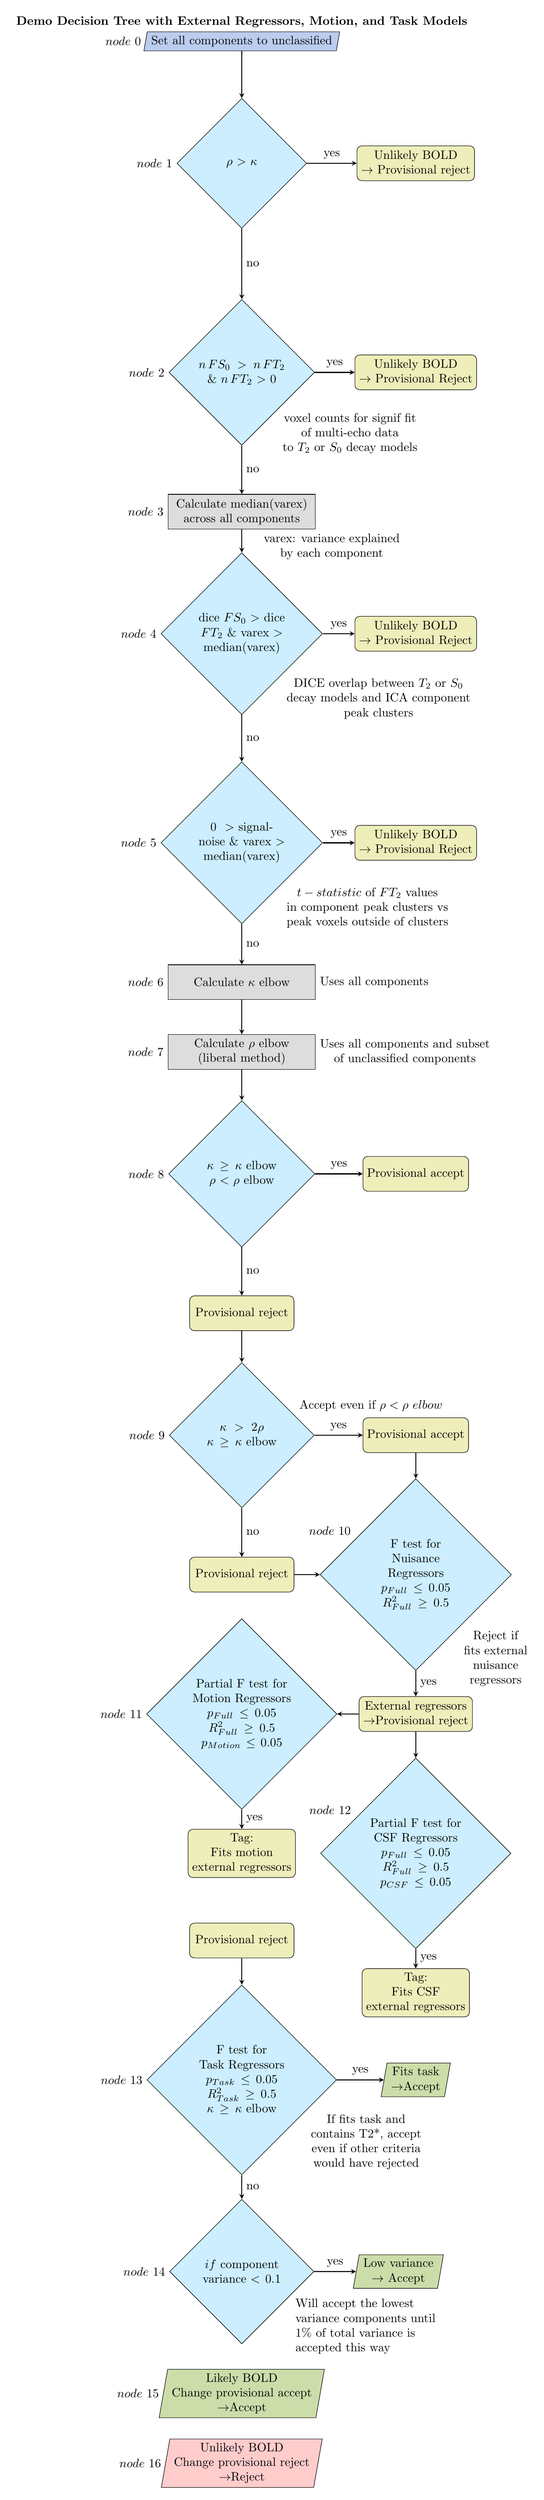
\begin{tikzpicture}[node distance = 2cm]

% ------------------------- nodes -------------------------
% ----- node: 0
\node(0)[input,label={90:\textbf{Demo Decision Tree with External Regressors, Motion, and Task Models}}, label={180:$node\ 0$}]{Set all components to unclassified};
% ----- node: 1
\node(1)[decision, below of=0,label={180:$node\ 1$}, yshift=-1.5cm]{$\rho$ $>$ $\kappa$};
\node(rej1)[changeclass, right of=1, xshift=3cm, align=center]{Unlikely BOLD\\$\rightarrow$ Provisional reject};
% ----- node: 2
\node(2)[decision, below of=1,label={180:$node\ 2$}, label={[align=center] 315: voxel counts for signif fit\\of multi-echo data\\to $T_2$ or $S_0$ decay models}, yshift=-4.0cm]{$n \, FS_0 \, > \, n \, FT_2$ \& $n \,FT_2$ $>$ 0};
\node(rej2)[changeclass, right of=2, xshift=3cm, align=center]{Unlikely BOLD\\$\rightarrow$ Provisional Reject};
% ----- node: 3
\node(3)[process, below of=2, label={180:$node\ 3$}, label={[align=center] 315: varex: variance explained\\by each component}, yshift=-2.0cm]{Calculate median(varex) across all components};
% ----- node: 4
\node(4)[decision, below of=3,label={180:$node\ 4$},label={[align=center] 315:DICE overlap between $T_2$ or $S_0$\\decay models and ICA component\\peak clusters}, yshift=-1.5cm]{dice $FS_0$ $>$ dice $FT_2$ \& varex $>$ median(varex)
};
\node(rej4)[changeclass, right of=4, xshift=3cm, align=center]{Unlikely BOLD\\$\rightarrow$ Provisional Reject};
% ----- node: 5
\node(5)[decision, below of=4,label={180:$node\ 5$}, label={[align=center] 315: $t-statistic$ of $FT_2$ values\\in component peak clusters vs\\peak voxels outside of clusters}, yshift=-4.0cm]{ $0 \, >$ signal-noise \&  varex $>$ median(varex)};
\node(rej5)[changeclass, right of=5, xshift=3cm, align=center]{Unlikely BOLD\\$\rightarrow$ Provisional Reject};
% ----- node: 6
\node(6)[process, below of=5, label={180:$node\ 6$}, label={0: Uses all components}, yshift=-2.0cm]{Calculate $\kappa$ elbow};
% ----- node: 7
\node(7)[process, below of=6, label={180:$node\ 7$}, label={[align=center] 0: Uses all components and subset\\of unclassified components}]{Calculate $\rho$ elbow\\(liberal method)};
% ----- node: 8
\node(8)[decision, below of=7,label={180:$node\ 8$}, yshift=-1.5cm]{$\kappa \geq \kappa$ elbow\\$\rho$ $<$ $\rho$ elbow};
\node(chrej8)[changeclass, below of=8, xshift=0cm, yshift=-2cm]{Provisional reject};
\node(chacc8)[changeclass, right of=8, xshift=3cm, yshift=0cm]{Provisional accept};
% ----- node: 9
\node(9)[decision, below of=chrej8,label={180:$node\ 9$},label={20: Accept even if $\rho < \rho\ elbow$},yshift=-1.5cm]{$\kappa > 2\rho$\\$\kappa \geq \kappa$ elbow};
\node(chrej9)[changeclass, below of=9, xshift=0cm, yshift=-2cm]{Provisional reject};
\node(chacc9)[changeclass, right of=9, xshift=3cm, yshift=0cm]{Provisional accept};
% ----- node: 10
\node(10)[decision, below of=chacc9,label={150:$node\ 10$},label={[align=center] 310: Reject if\\fits external\\nuisance\\regressors},yshift=-2cm]{F test for\\Nuisance Regressors\\$p_{Full} \leq 0.05$\\$R^2_{Full} \geq 0.5$};
\node(chrej10)[changeclass, below of=10, xshift=0cm, yshift=-2cm, align=center]{External regressors\\$\rightarrow$Provisional reject};
% ----- node: 11
\node(11)[decision, left of=chrej10,label={180:$node\ 11$},xshift=-3cm]{Partial F test for\\Motion Regressors\\$p_{Full} \leq 0.05$\\$R^2_{Full} \geq 0.5$\\$p_{Motion} \leq 0.05$};
\node(chtag11)[changeclass, below of=11, xshift=0cm, yshift=-2cm, align=center]{Tag:\\Fits motion\\external regressors};
% ----- node: 12
\node(12)[decision, below of=chrej10,label={150:$node\ 12$},yshift=-2cm]{Partial F test for\\CSF Regressors\\$p_{Full} \leq 0.05$\\$R^2_{Full} \geq 0.5$\\$p_{CSF} \leq 0.05$};
\node(chtag12)[changeclass, below of=12, xshift=0cm, yshift=-2cm, align=center]{Tag:\\Fits CSF\\external regressors};
% ----- node: 13
\node(prej13)[changeclass, below of=chtag11, xshift=0cm, yshift=-0.5cm]{Provisional reject};
\node(13)[decision, below of=prej13,label={180:$node\ 13$},label={[align=center] 335: If fits task and\\contains T2*, accept\\even if other criteria\\would have rejected},yshift=-2cm]{F test for\\Task Regressors\\$p_{Task} \leq 0.05$\\$R^2_{Task} \geq 0.5$\\$\kappa \geq \kappa$ elbow};
\node(chacc13)[accept, right of=13,xshift=3cm, align=center]{Fits task\\$\rightarrow$Accept};
% ----- node: 14
\node(14)[decision, below of=13,label={180:$node\ 14$},label={[align=left] 335: Will accept the lowest\\variance components until\\1\% of total variance is\\accepted this way}, yshift=-3.5cm]{$if$ component variance $<0.1$};%--check in kundu
\node(acc14)[accept, right of=14, xshift=2.5cm, align=center]{Low variance\\$\rightarrow$ Accept};
% ----- node: 15
\node(15)[accept, below of=14,label={180:$node\ 15$},yshift=-1.5cm, align=center]{Likely BOLD\\Change provisional accept\\$\rightarrow$Accept};
% ----- node: 16
\node(16)[reject, below of=15,label={180:$node\ 16$}, yshift=0cm, align=center]{Unlikely BOLD\\Change provisional reject\\$\rightarrow$Reject};

% ------------------------- connections -------------------------
% draw[x](origin)--node[anchor=position]{text}(destination);
\draw[arrow](0)--(1);
\draw[arrow](1)--node[anchor=south, right=0] {no} (2);
\draw[arrow](1)--node[anchor=south] {yes} (rej1);
\draw[arrow](2)--node[anchor=south, right=0] {no} (3);
\draw[arrow](2)--node[anchor=south] {yes} (rej2);
\draw[arrow](3)--(4);
\draw[arrow](4)--node[anchor=south, right=0] {no} (5);
\draw[arrow](4)--node[anchor=south] {yes} (rej4);
\draw[arrow](5)--node[anchor=south, right=0] {no} (6);
\draw[arrow](5)--node[anchor=south] {yes} (rej5);
\draw[arrow](6)--(7);
\draw[arrow](7)--(8);
\draw[arrow](8)--node[anchor=south] {yes} (chacc8);
\draw[arrow](8)--node[anchor=south, right=0] {no} (chrej8);
\draw[arrow](chrej8)--(9);
\draw[arrow](9)--node[anchor=south] {yes} (chacc9);
\draw[arrow](9)--node[anchor=south, right=0] {no} (chrej9);
\draw[arrow](chacc9)--(10);
\draw[arrow](chrej9)--(10);
\draw[arrow](10)--node[anchor=south, right=0] {yes} (chrej10);
\draw[arrow](chrej10)--(11);
\draw[arrow](11)--node[anchor=south, right=0] {yes} (chtag11);
\draw[arrow](chrej10)--(12);
\draw[arrow](12)--node[anchor=south, right=0] {yes} (chtag12);
\draw[arrow](prej13)--(13);
\draw[arrow](13)--node[anchor=south] {yes} (chacc13);
\draw[arrow](13)--node[anchor=south, right=0] {no} (14);
\draw[arrow](14)--node[anchor=south] {yes} (acc14);
\end{tikzpicture}
\end{document}
